%%%%%%%%%%%%%%%%%%%%%%%%%%%%%%%%%%%%%%%%%%%%%%%%%%%%%%%%%%%%%%%%%%%%%%%%%%
 %																		%
 %	Plantilla Latex para presentación del proyecto de curso				%
 %	Programación de Aplicaciones para Internet y la Nube					%
 %		
 																%
 %	              Creada por: Duván Pardo, Wilson López								%
 %					
 %  Modificada por: Pedro J. Vargas Barrios					
 %		                                                                              %
 %	Versión: 0.2															%
 %	Dapardoc@gmail.com ; Wilrilo@gmail.com								%
 %																		% 
 %	Se requieren los archivos  plantilla.bbl								% 
 %	El directorio Imagenes que contiene: CECAD,DC, Elementos y RITA		%  
 %																		%
%%%%%%%%%%%%%%%%%%%%%%%%%%%%%%%%%%%%%%%%%%%%%%%%%%%%%%%%%%%%%%%%%%%%%%%%%%

\documentclass[10pt]{article}\usepackage[]{graphicx}\usepackage[]{color}
%% maxwidth is the original width if it is less than linewidth
%% otherwise use linewidth (to make sure the graphics do not exceed the margin)
\makeatletter
\def\maxwidth{ %
  \ifdim\Gin@nat@width>\linewidth
    \linewidth
  \else
    \Gin@nat@width
  \fi
}
\makeatother

\definecolor{fgcolor}{rgb}{0.345, 0.345, 0.345}
\newcommand{\hlnum}[1]{\textcolor[rgb]{0.686,0.059,0.569}{#1}}%
\newcommand{\hlstr}[1]{\textcolor[rgb]{0.192,0.494,0.8}{#1}}%
\newcommand{\hlcom}[1]{\textcolor[rgb]{0.678,0.584,0.686}{\textit{#1}}}%
\newcommand{\hlopt}[1]{\textcolor[rgb]{0,0,0}{#1}}%
\newcommand{\hlstd}[1]{\textcolor[rgb]{0.345,0.345,0.345}{#1}}%
\newcommand{\hlkwa}[1]{\textcolor[rgb]{0.161,0.373,0.58}{\textbf{#1}}}%
\newcommand{\hlkwb}[1]{\textcolor[rgb]{0.69,0.353,0.396}{#1}}%
\newcommand{\hlkwc}[1]{\textcolor[rgb]{0.333,0.667,0.333}{#1}}%
\newcommand{\hlkwd}[1]{\textcolor[rgb]{0.737,0.353,0.396}{\textbf{#1}}}%

\usepackage{framed}
\makeatletter
\newenvironment{kframe}{%
 \def\at@end@of@kframe{}%
 \ifinner\ifhmode%
  \def\at@end@of@kframe{\end{minipage}}%
  \begin{minipage}{\columnwidth}%
 \fi\fi%
 \def\FrameCommand##1{\hskip\@totalleftmargin \hskip-\fboxsep
 \colorbox{shadecolor}{##1}\hskip-\fboxsep
     % There is no \\@totalrightmargin, so:
     \hskip-\linewidth \hskip-\@totalleftmargin \hskip\columnwidth}%
 \MakeFramed {\advance\hsize-\width
   \@totalleftmargin\z@ \linewidth\hsize
   \@setminipage}}%
 {\par\unskip\endMakeFramed%
 \at@end@of@kframe}
\makeatother

\definecolor{shadecolor}{rgb}{.97, .97, .97}
\definecolor{messagecolor}{rgb}{0, 0, 0}
\definecolor{warningcolor}{rgb}{1, 0, 1}
\definecolor{errorcolor}{rgb}{1, 0, 0}
\newenvironment{knitrout}{}{} % an empty environment to be redefined in TeX

\usepackage{alltt}   			% Describe el tipo de documento, y el tamaño de la letra del texto

\usepackage[utf8]{inputenc}				% Define codificación para que permita caracteres latinos (acentos)
\usepackage[spanish,activeacute]{babel} 	% Paquete para poder escribir con tildes y otros caracteres especiales
\usepackage{amsmath}

\usepackage{vmargin}						% Código para margenes y formato de página
\setpapersize{A4}
\setmargins	{2.2cm}     					% margen izquierdo
			{1 cm}                 		% margen superior
			{16.5cm}               		% anchura del texto
			{23.42cm}             		% altura del texto
			{20pt}                		% altura de los encabezados
			{1.2cm}               		% espacio entre el texto y los encabezados
			{0pt}                		% altura del pie de página
			{2cm}                 		% espacio entre el texto y el pie de página

\usepackage{amsmath}						% paquete para expresiones matemáticas
					% paquete para escritura de ecuaciones 
\usepackage{amssymb}						% paquete para caracteres especiales para ecuaciones 
\usepackage[export]{adjustbox}


\usepackage{fancyhdr}					% Temas para encabezado y pie de pagina
\usepackage{fancyvrb}
\pagestyle{fancy} 

\pagenumbering{arabic} 					% Numeración de paginas {arabic roman}
\usepackage{hyperref}					% Para hipervinculos
\usepackage{graphicx}					% Para incluir imágenes
\usepackage{caption}						% Descripciones de las figuras
\usepackage{subcaption}					% Descripción varias imagenes en usa sola figura
\graphicspath{ {Imagenes/} }				% Directorio de imágenes esta capeta va donde esta el archivo tex


\usepackage{color, colortbl}				% Colores para tablas
	
\usepackage{framed, color}              % Para cuadro de texto - Pedro Vargas
\usepackage{listings}					% Para el código Fuente
\usepackage{xcolor}		                  % para color en codigos o listrings
\definecolor{shadecolor}{rgb}{1,0.89,0.6}				%  % Para cuadro de texto - Pedro Vargas
\definecolor{limegreen}{RGB}{50,100,50}	% Definición de colores ejemplo verde en RGB
\definecolor{Red}{RGB}{220,120,120}		% se definen colores para la tabla en el cronograma pueden ser RGB 0-255 o rgb 0-1 cada componente
\definecolor{LightCyan}{rgb}{0.88,1,1}
\definecolor{azul}{RGB}{120,120,210}
\lstdefinestyle{base}{
	language=C,
	emptylines=1,
	breaklines=true,
	showspaces=fasle,
	showstringspaces=false,
	extendedchars=true,
	basicstyle=\ttfamily\color{black},
	moredelim=**[is][\color{limegreen}]{'}{'}, 	% Para este caso especial el caracter ' y & encierran
	moredelim=**[is][\color{blue}]{&}{&},		% un fragmento de código que quiere ser coloreado
}

\lstset{numbers=left, numberstyle=\tiny, stepnumber=2, numbersep=5pt}

%Aquí inicia el documento.
\IfFileExists{upquote.sty}{\usepackage{upquote}}{}
\begin{document}
	% Se define el Encabezado
	%clhead[]{Proyecto}
	\lhead[]{Proyecto Final - Generación de contenido académico mediante R}
	\rhead[]{\textbf{2016-I}}
	\renewcommand{\headrulewidth}{0.5pt}

	\thispagestyle{empty}						% La primera página no lleva estilo (sin encabezado)
	\begin{center}
		\large {Proyecto Final - Desarrollo de aplicación para la generación de contenido académico mediante R\\
			\hspace{0 cm}\textbf{2016-I}}
		\bigskip  
		\textbf{
			\LARGE{\\Desarrollo de aplicación para la generación de contenido académico mediante R}}\\								% Nombre del proyecto
	\end{center}	
	\begin{flushright}	
		\bigskip	
		Nombre del Estudiante: \textbf{Pedro J. Vargas Barrios}			% Nombre del estudiante
	\end{flushright} 
	
	
	
	\section{Introducción}

La generación de informes dinámicos a partir de la programación literaria es resultado de la propuesta de Donald Knuth, quien la propuso como una alternativa al tradicional paradigma de la programación estructurada. Con este enfoque el autor/investigador puede plantear sus ideas, ecuaciones o demás métodos que requieran algún tipo de cálculo, y, con ello, mediante código R obtener facilidad para modificar o replicar sus propuestas de investigación.\\
La forma de identificar y manipular los datos en el documento contribulle a una rápida comprensión de lo que se expone en él, sin importar la temática. En el presente proyecto se tomará el tema de fundamentos de circuitos para proponer una alternativa que ayude a manipular de forma sencilla la información requerida de esta materia y a la vez que esté soportada en un servicio en la nube.
 
\section{Descripción del proyecto}

El proyecto busca hacer uso de los servicios de la nube y aprovechar las características de la programación literaria, ambos orientados hacia la elaboración de materíal técnico/académico en un determinado tema, en este caso fundamentos de circuitos. \\
Se parte de un documento en LaTeX relacionado con el tema de fundamentos de circuitos que obtiene los valores de los ejemplos incluidos en él de una base de datos que estará sobre Amazon Web Service. En principio tendrá unos valores por defecto para evitar errores durante su ejecución, posteriormente el usuario tendrá la opción de modificar el contenido de los ejemplos y gráficas del documento sin tener que ingresar a revisar el código en LaTeX a profundidad, es decir que no deberá requerir grandes conocimientos en esta área, sino que podrá concentrarse en el tema del documento (fundamentos de circuitos) que quiere consultar o generar, lo cual resulta de gran ventaja para textos extensos. Esta modificación la realizará mediante una aplicación que tomará los datos tomados por el usuario, los dejará en la nube y, a partir de estos se podrá generar el documento con R que deberá conectarse con este servidor.\\

\section{Objetivos}

\subsection{General}

	\begin{itemize}
		\item Desarrollar una aplicación que permita presentar mediante LaTeX y R, utilizar material académico y práctico para exponer fundamentos de circutos eléctricos.
	\end{itemize}
	
\subsection{Especificos}

\begin{itemize}
\item Desarrollar una aplicación  que permita presentar mediante LaTeX y R, utilizar material académico y práctico para exponer fundamentos de circuitos.
\end{itemize}
\begin{itemize}
\item Definir un conjunto de circuitos utilizar para presentar los ejercicios académicos del documento.
\end{itemize}
\begin{itemize}
\item Estructurar mediante programación literaria las reglas de los resultados de los ejercicios prácticos propuestos.
\end{itemize}
	

\section{Desarrollo del Proyecto}

\subsection{Configuración de servidor ec2}
Se desplegó un servidor en AWS con una base de datos MySQL y un servidor en apache sobre el que se montaría la aplicación web. Con estas características, el servidor
soporta la interacción del usuario con la base de datos y cuando se requiera, permitirá la conexión co R para realizar las operaciones necesarias.

\subsection{Características aplicación web}
La aplicación web se desarrolló en PHP, tiene un conjunto de opciones sobre los diferentes capítulos que permite modificar la información de la base de datos. Esta debe tener información relacionada con el desarrollo del contenido en R Studio.

\subsection{Desarrollo en R Studio}
EL documento en R tiene la estructura e información de un libro común, sin embargo tiene la particularidad de que su contenido puede ser modificado a través de la pagina web. Tiene una conexión a la base de datos en la cual se guardan los datos que un usuario remotamente asigna.

\newpage

\section{Resultados del proyecto - Fundamentos de Circuitos}

	\subsection{Introducción}
	
	\subsection{Capítulo 1 - Resistencias en Serie}
	
	\subsubsection{Ejercios resueltos capitulo 1}
	\begin{enumerate}
\item Calcular la resistencia total a partir del siguiente grupo de resistencias en serie.\\

\begin{figure}[h!] % Es preferible verificar la documentación para que la imagen quede correctamente segun el parámetro entre []
	\centering
		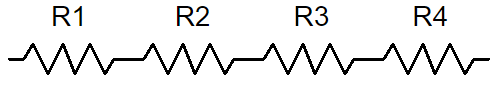
\includegraphics[scale=0.6]{Imagenes/cap1_ej1_res_serie.png}   
	\caption{Ejercicio 1 - Resistencias en serie} \label{fig:cap1_ej1_res_serie.png}
\end{figure}

Los valores de las resistencias \textbf{en ohmios}  son los siguientes:
\begin{knitrout}
\definecolor{shadecolor}{rgb}{0.969, 0.969, 0.969}\color{fgcolor}\begin{kframe}
\begin{verbatim}
## Valor_R1 Valor_R2 Valor_R3 Valor_R4 
##      600      400      200      300
\end{verbatim}
\end{kframe}
\end{knitrout}

\textbf{Respueta: }El valor total de las resistencias en serie es:
\begin{knitrout}
\definecolor{shadecolor}{rgb}{0.969, 0.969, 0.969}\color{fgcolor}\begin{kframe}
\begin{verbatim}
## [1] 1500
\end{verbatim}
\end{kframe}
\end{knitrout}

\item Calcular la resistencia total \textbf{en kiloohmios y ohmios} del siguiente grupo de resistencias:\\

\begin{figure}[h!] % Es preferible verificar la documentación para que la imagen quede correctamente segun el parámetro entre []
	\centering
		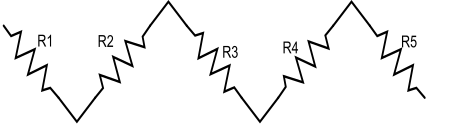
\includegraphics[scale=1.5]{Imagenes/cap1_ej2_res_serie.png}   
	\caption{Ejercicio 2 - Resistencias en serie} \label{fig:cap1_ej2_res_serie.png}
\end{figure}

Los valores de las resistencias \textbf{en Kiloohmios}  son los siguientes:
\begin{knitrout}
\definecolor{shadecolor}{rgb}{0.969, 0.969, 0.969}\color{fgcolor}\begin{kframe}
\begin{verbatim}
## Valor_R1 Valor_R2 Valor_R3 Valor_R4 Valor_R5 
##        4        5        6        7        8
\end{verbatim}
\end{kframe}
\end{knitrout}

\textbf{Respueta: }El valor total de las resistencias en serie es:\\
En kiloohmios:
\begin{knitrout}
\definecolor{shadecolor}{rgb}{0.969, 0.969, 0.969}\color{fgcolor}\begin{kframe}
\begin{verbatim}
## [1] 30
\end{verbatim}
\end{kframe}
\end{knitrout}
En Ohmios:
\begin{knitrout}
\definecolor{shadecolor}{rgb}{0.969, 0.969, 0.969}\color{fgcolor}\begin{kframe}
\begin{verbatim}
## [1] 30000
\end{verbatim}
\end{kframe}
\end{knitrout}


\item Calcular la resistencia total \textbf{en kiloohmios y ohmios} del circuito de la imagen:\\

\begin{figure}[h!] % Es preferible verificar la documentación para que la imagen quede correctamente segun el parámetro entre []
	\centering
		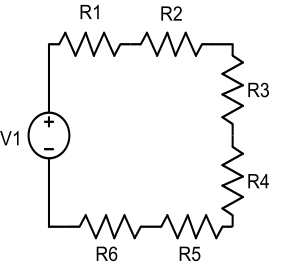
\includegraphics[scale=1.9]{Imagenes/cap1_ej3_res_serie.png}   
	\caption{Ejercicio 3 - Resistencias en serie} \label{fig:cap1_ej3_res_serie.png}
\end{figure}

Los valores de las resistencias \textbf{en Kiloohmios}  son los siguientes:
\begin{knitrout}
\definecolor{shadecolor}{rgb}{0.969, 0.969, 0.969}\color{fgcolor}\begin{kframe}
\begin{verbatim}
## Valor_R1 Valor_R2 Valor_R3 Valor_R4 Valor_R5 Valor_R6 
##       45       34       56       23       96       65
\end{verbatim}
\end{kframe}
\end{knitrout}

\textbf{Respueta: }El valor total de las resistencias en serie es:\\
En kiloohmios:
\begin{knitrout}
\definecolor{shadecolor}{rgb}{0.969, 0.969, 0.969}\color{fgcolor}\begin{kframe}
\begin{verbatim}
## [1] 319
\end{verbatim}
\end{kframe}
\end{knitrout}
En Ohmios:
\begin{knitrout}
\definecolor{shadecolor}{rgb}{0.969, 0.969, 0.969}\color{fgcolor}\begin{kframe}
\begin{verbatim}
## [1] 319000
\end{verbatim}
\end{kframe}
\end{knitrout}

\newpage 



\end{enumerate}
	

	
	\subsection{Capítulo 2 - Resistencias en Paralelo}
	
	\subsubsection{Ejercios resueltos capitulo 2}
	\begin{enumerate}
\item Calcular la resistencia total a partir de las siguientes resistencias en paralelo:\\

\begin{figure}[h!] % Es preferible verificar la documentación para que la imagen quede correctamente segun el parámetro entre []
	\centering
		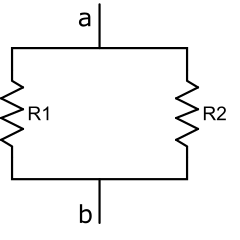
\includegraphics[scale=1.9]{Imagenes/cap2_ej1_res_paral.png}   
	\caption{Ejercicio 1 - Resistencias en paralelo} \label{fig:cap2_ej1_res_paral.png}
\end{figure}



Los valores de las resistencias son: R1= 555 $\Omega$, R2= 444 $\Omega$ \\

Con lo cual quedaría:\\
{\LARGE $ \frac{1}{Req} =  \frac{1}{R1} + \frac{1}{R2}  $}\\

{\LARGE $ \frac{1}{Req} =  \frac{1}{ 555} + \frac{1}{444}  $}\\



 $Req = 246.6666667$\\

\item Calcular la resistencia total entre a y b:\\

\begin{figure}[h!] % Es preferible verificar la documentación para que la imagen quede correctamente segun el parámetro entre []
	\centering
		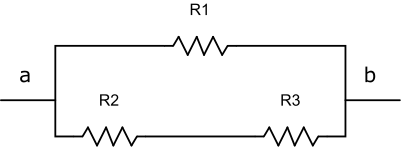
\includegraphics[scale=1]{Imagenes/cap2_ej2_res_paral.png}   
	\caption{Ejercicio 2 - Resistencias serie-paralelo} \label{fig:cap2_ej2_res_paral.png}
\end{figure}



Los valores de las resistencias son: R1= 200 $\Omega$, R2= 150 $\Omega$, , R3= 50 $\Omega$ \\
Se suma R2 y R3 para obtener R4.\\


$R4 = R2 + R3$\\
$R4 = 150 + 50$\\
$R4 = 200$\\

\begin{figure}[h!] % Es preferible verificar la documentación para que la imagen quede correctamente segun el parámetro entre []
	\centering
		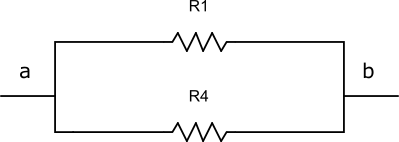
\includegraphics[scale=1]{Imagenes/cap2_ej2_res_paral_1.png}   
	\caption{Ejercicio 2 - Resistencias serie-paralelo} \label{fig:cap2_ej2_res_paral_1.png}
\end{figure}

Se suman las resistencias en paralelo R1=200 y R4=200\\

{\LARGE $ \frac{1}{Req} =  \frac{1}{R1} + \frac{1}{R4}  $}\\

{\LARGE $ \frac{1}{Req} =  \frac{1}{ 200} + \frac{1}{200}  $}\\



 $Req = 100$\\

 \item Calcular la resistencia total entre los puntos a y b del siguiente diagrama:
 
 \begin{figure}[h!] % Es preferible verificar la documentación para que la imagen quede correctamente segun el parámetro entre []
	\centering
		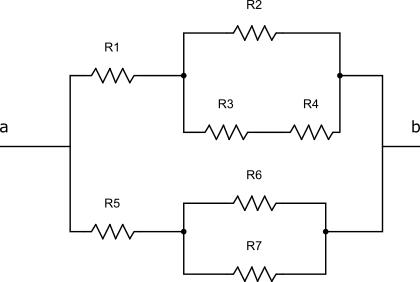
\includegraphics[scale=1]{Imagenes/cap2_ej3_res_paral.png}   
	\caption{Ejercicio 3 - Resistencias serie-paralelo} \label{fig:ccap2_ej3_res_paral.png}
\end{figure}
 

Los valores de las resistencias son: R1=45, R2=67, R3=13, R4=38, R5=3, R6=9, R7=56.\\



R3R4= R3 + R4\\
R3R4= 13+ 38\\
R3R4= 51\\\\

Sumar las resistencias R6 Y R7 en paralelo\\



R6R7= 1 / (1/R6+1/R7)\\
R6R7= 7.7538462\\\\

Sumar las resistencias en paralelo R2=67 y R3R4=51\\



R2R3R4= 1 / (1/R6+1/R7)\\
R2R3R4= R6R7= 28.9576271\\\\

La resistencia equivalente sería finalmente:

RT= R1+ R2R3R4 + R6R7 + R5


RT= 84.7114733

\end{enumerate}
	
	\subsection{Capitulo 3}
	

  \newpage
  
\section{Trabajos Futuros }
Creación de libros completos que sean modificables con facilidad\\
Modificación de contenido de papers en ponencias\\
Modificación de documentos mediante aplicaciones móviles



\end{document}
